% Drawing 122/01-4 -- folder 122, batch 01, archive page 8 (PDF page 9).
% Transcription: à gauche, un croquis : un disque marqué « $P$ », entouré d'un anneau hachuré ; à droite de l'anneau, « $\widetilde{P}$ ».
% Kind: disc inside a hatched annulus. Method 2 (schematic redraw from the facsimile). Status: ok.
% Notes: Two nested closed curves drawn freehand, the ring between them hatched with short oblique strokes; P inside the inner curve, P-tilde to the right of the outer one. The outer curve is an oval leaning to the right, wider at the bottom left; the inner one is open at the upper left, where a separate stroke continues it and a heavy stroke doubles the outer curve. Outside the ring on the right, a curved stroke runs from the top down and round the lower right of the outer curve, with a short tail rising from it towards P-tilde; drawn as on the page. The hatching: short strokes in the upper band, long oblique strokes in the left and lower bands, a few in the right band. Overlaid 2026-11-12 (Opus 5.5) on a 400 dpi colour render: the earlier redraw drew two circles with radial hatching, which did not match the leaning ovals of the page; the curves, the hatching, the right-hand stroke and its tail are now traced through points measured on the page. The transcription's note matches. Redrawn 2026-11-12 (issue 128): to check again.
% Coordinates: 1 unit = 1 mm = 1/100 of the crop width (bbox in page fractions: [0.12, 0.36, 0.33, 0.5]).
% Redrawn by Claude (claude-fable-5-2), issue #128, 2026-11-12; not checked by a human; not compiled (no TeX in the session).
% Overlaid by Claude (claude-opus-5-5) 2026-11-12 (issue #128): rasterised from its own coordinates over the colour facsimile and checked or corrected. Not compiled. Status: ok.
% Rights: reproduces part of the work -- behind RENDER_TRANSCRIPTS, never published by itself.
\documentclass[tikz,border=3pt]{standalone}
\usepackage{amsmath,amssymb}
\usetikzlibrary{patterns,arrows.meta}
\tikzset{pencil/.style={black!45}, struck/.style={black!35}, mpt/.style={circle,draw,inner sep=1.3pt}, pt/.style={circle,fill,inner sep=0.9pt}, opt/.style={circle,draw,fill=white,inner sep=1.1pt}}
\begin{document}
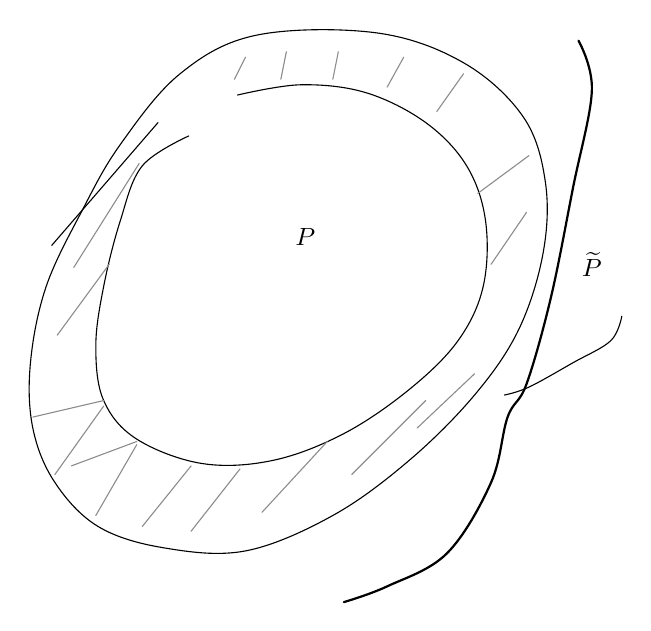
\begin{tikzpicture}[x=1mm,y=1mm,line cap=round,line join=round,font=\scriptsize]
\draw plot[smooth cycle, tension=0.6] coordinates {(41,-11.9) (56.2,-11.6) (67.3,-15.4) (74.9,-22.3) (77.7,-30.6) (77.4,-39.6) (74.3,-49.3) (68.7,-57.6) (60.4,-65.9) (50.7,-72.9) (39.6,-77.4) (29.2,-77) (20.9,-74.3) (15.4,-68.7) (12.6,-61.8) (12.3,-53.5) (14.3,-43.8) (18.9,-34.1) (23.7,-25.8) (31.3,-16.8)};
\draw plot[smooth, tension=0.6] coordinates {(38.6,-19.5) (46.6,-18.2) (54.9,-19.2) (62.5,-23) (67.7,-28.5) (70.1,-35.5) (69.8,-43.8) (66.6,-50.7) (60.4,-56.9) (52.1,-62.5) (43.1,-65.9) (34.1,-66.3) (25.8,-63.2) (21.6,-58.3) (20.6,-51.4) (21.6,-43.8) (23.7,-35.5) (26.5,-28.5) (32.4,-24.7)};
\draw (15,-38.6) -- (28.5,-23);
\draw[pencil] (38.2,-17.5) -- (39.6,-14.7);
\draw[pencil] (44.1,-17.5) -- (44.8,-14);
\draw[pencil] (50.7,-17.5) -- (51.4,-14);
\draw[pencil] (57.6,-18.5) -- (59.7,-14.7);
\draw[pencil] (63.9,-21.6) -- (67.3,-16.8);
\draw[pencil] (17.8,-41.4) -- (26.1,-28.2);
\draw[pencil] (15.7,-50) -- (22.3,-41);
\draw[pencil] (12.6,-60.4) -- (21.6,-58.3);
\draw[pencil] (15.4,-67.7) -- (21.6,-59);
\draw[pencil] (17.5,-66.6) -- (25.8,-63.5);
\draw[pencil] (20.6,-72.9) -- (25.8,-63.9);
\draw[pencil] (26.5,-74.3) -- (32.7,-66.6);
\draw[pencil] (32.7,-74.9) -- (38.9,-67);
\draw[pencil] (41.7,-72.5) -- (50,-63.5);
\draw[pencil] (53.1,-67.7) -- (62.5,-58.3);
\draw[pencil] (61.4,-61.8) -- (68.7,-54.9);
\draw[pencil] (69.1,-32) -- (75.6,-27.2);
\draw[pencil] (70.8,-41) -- (75.3,-34.4);
\draw[thick] plot[smooth, tension=0.6] coordinates {(81.9,-12.6) (83.6,-18.9) (81.2,-31.3) (78.4,-45.2) (75.3,-56.2) (72.9,-60.4) (70.8,-68.7) (65.2,-77.7) (57.6,-81.9) (52.1,-83.9)};
\draw plot[smooth, tension=0.6] coordinates {(72.5,-57.6) (75.6,-56.6) (81.2,-53.5) (86,-50.7) (87.4,-47.6)};
\node[inner sep=1pt] at (47.2,-37.5) {\small $P$};
\node[inner sep=1pt] at (83.6,-41) {\small $\widetilde{P}$};
\end{tikzpicture}
\end{document}
